\documentclass[11pt,a4paper]{article}

\usepackage[margin=1in]{geometry}
\usepackage{amsmath,amssymb}
\usepackage{graphicx}
\usepackage{booktabs}
\usepackage{hyperref}
\usepackage{natbib}
\usepackage{xcolor}

\title{Generative denoising for template-free gravitational-wave burst search}
\author{
  Panagiotis Minoglou\thanks{Independent researcher.
  Corresponding author. E-mail: \texttt{panosmng97@gmail.com}}
}
\date{\today}

\begin{document}
\maketitle

\begin{abstract}
Binary black hole (BBH) deep classifiers such as AresGW are optimized for
compact-binary morphologies in a fixed mass range. Unmodeled transients
(e.g.\ core-collapse supernovae and other short bursts) lie outside that
training objective. We present Keno, a generative residual-search pipeline that
learns detector noise, subtracts the predicted noise from whitened strain, and
searches the residual with template-free excess power, dual-interferometer
coherent lag scans, and an envelope-consistency glitch veto.
On unknown-morphology injections in real LIGO noise at 1\% false-alarm rate,
Keno residual excess power saturates near 100\% efficiency across SNR\,2--12,
while a BBH-trained AresGW-class ResNet plateaus near 60--80\% and mismatched
matched filtering remains near 20\%.
On published GWTC/cWB GPS times, coherent residual coincidence recovers 9/18
dual-detector events after vetoing the known L1 glitch contamination of GW170817.
Keno is complementary to AresGW: it does not claim superior BBH sensitive
distance in the AresGW mass range.
\end{abstract}

\section{Introduction}

Matched filtering and BBH-trained deep networks dominate compact-binary
searches~\citep{nousi2023,koloniari2025}.
AresGW~\citep{nousi2023} uses a deep residual network with adaptive
normalization to classify one-second segments as BBH or noise, achieving
competitive sensitive distances in its training mass window.
That success does not transfer to morphologies absent from training.

Unmodeled burst searches (e.g.\ coherent WaveBurst) ask a different question:
whether excess coherent power remains after accounting for detector noise.
Keno follows that spirit with a generative step: a 1D U-Net predicts
instrumental noise $N$, forming
\begin{equation}
S_{\mathrm{clean}} = S_{\mathrm{raw}} - \hat N,
\end{equation}
then applies template-free excess power on $S_{\mathrm{clean}}$.

\paragraph{Claim scope.}
We claim superiority on \emph{unknown-morphology} bursts at controlled false-alarm
rate. We do \emph{not} claim that Keno supersedes AresGW on BBH detection.

\section{Method}

Figure~\ref{fig:pipeline} summarizes the production path. All strain segments
are whitened and sampled at $f_s=4096\,\mathrm{Hz}$. Unless noted, analysis
windows are $T=4\,\mathrm{s}$ ($N=16\,384$ samples).

\begin{figure}[t]
  \centering
  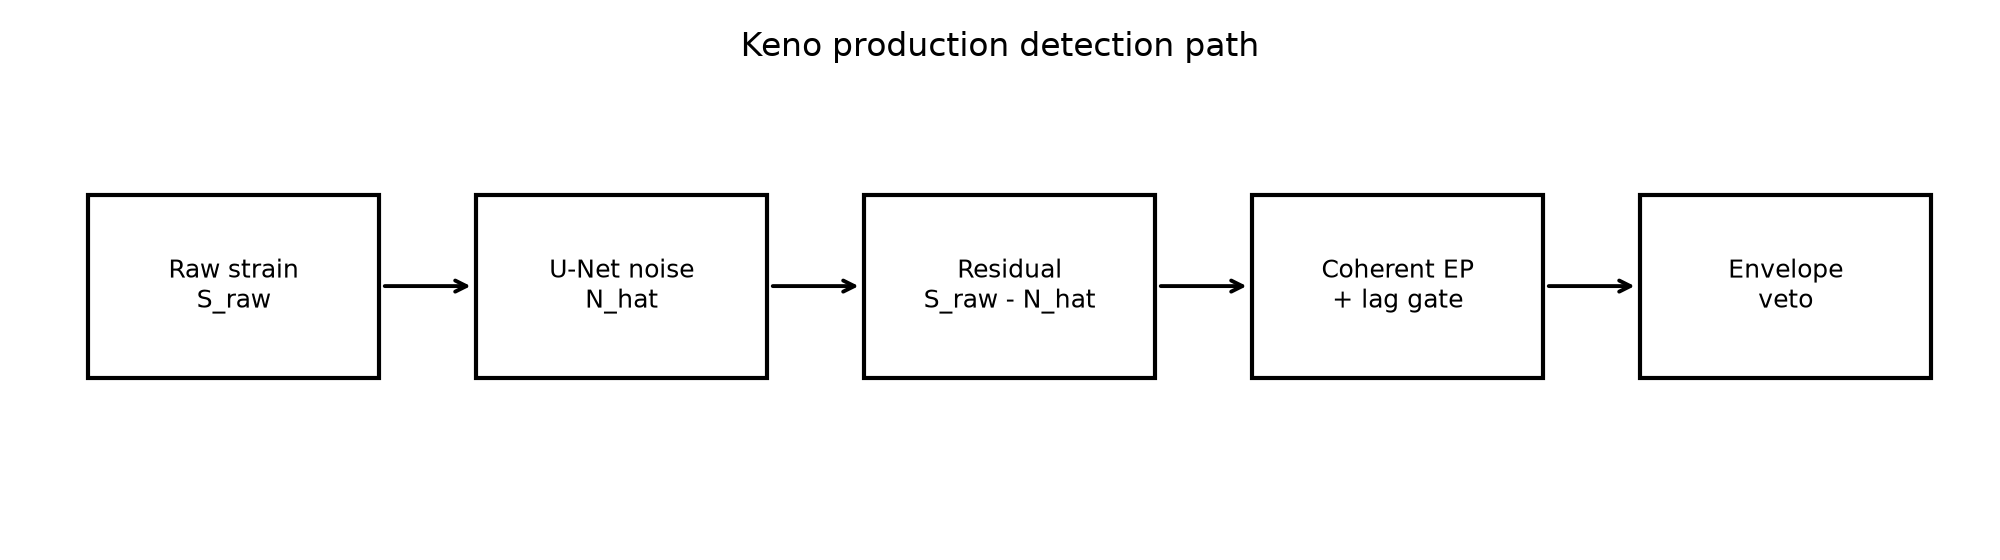
\includegraphics[width=0.95\linewidth]{figures/fig1_pipeline.png}
  \caption{Keno production detection path: generative noise subtraction,
  residual excess power, coherent H1+L1 lag scan, and envelope-consistency veto.}
  \label{fig:pipeline}
\end{figure}

\subsection{Generative noise model}
Keno uses a 1D U-Net noise denoiser~\cite{ronneberger2015} with four
encoder/decoder stages (base width 16 channels, kernel size 9, GELU
activations and batch normalization). The network maps whitened strain
$S_{\mathrm{raw}}$ to a predicted noise waveform $\hat N$ and forms the
residual
\begin{equation}
R = S_{\mathrm{raw}} - \hat N.
\end{equation}
Training uses real GWOSC background windows cached for H1/L1. Fine-tuning
emphasizes burst preservation so that injected short transients survive
subtraction. A Phase-1 hold-out check requires mean normalized recovery error
$\mathrm{RMS}(R-s)/\mathrm{RMS}(s)<0.15$ on injected bursts with known ground
truth $s$. The production checkpoint for this work is frozen under label
\texttt{2026-07-paper-v1} (SHA256 prefix \texttt{55ce7637\ldots}).

\subsection{Template-free excess-power statistic}
On a residual (or raw) time series $x(t)$, Keno computes a short-time Fourier
transform (Hann window, $n_{\mathrm{perseg}}=256$, 75\% overlap), forms
bin power $P(f,t)$, estimates a robust noise floor as the median of $P$, and
defines the detection statistic as the peak normalized excess power
\begin{equation}
\rho_{\mathrm{EP}}(x)
  = \max_{f,t}\frac{P(f,t)}{\mathrm{median}(P)}.
\end{equation}
This is a cWB-style, morphology-agnostic energy excess measure: no template
inner product is required.

\subsection{Single-detector residual search}
For a single interferometer, Keno reports $\rho_{\mathrm{EP}}(R)$ and
compares it to a threshold $\theta_{\mathrm{IFO}}$ calibrated on noise-only
windows at a target false-alarm rate (FAR). Calibration uses the empirical
$(1-\mathrm{FAR})$ percentile after trimming the upper 1\% of
subtraction-glitched noise trials (artifact-robust threshold). In the freeze,
$\theta_{\mathrm{IFO}}\approx 4004.6$ at 1\% FAR. This gate is used for
single-IFO diagnostics and independent residual coincidence; dual-IFO
\emph{production} detection uses the coherent threshold below.

\subsection{Coherent dual-IFO lag scan}
For H1 and L1 residuals $R_{\mathrm{H}}$ and $R_{\mathrm{L}}$, Keno scans
integer sample lags $\ell$ with $|\ell|/f_s \le \Delta t_{\mathrm{lag}}$
($\Delta t_{\mathrm{lag}}=10\,\mathrm{ms}$, the approximate light-travel
window between sites) and polarities $p\in\{+1,-1\}$, forming
\begin{equation}
C_{\ell,p}
  = \frac{R_{\mathrm{H}} + p\,\mathcal{S}_{\ell}(R_{\mathrm{L}})}{\sqrt{2}},
\end{equation}
where $\mathcal{S}_{\ell}$ is a zero-padded shift. The coherent statistic is
\begin{equation}
\rho_{\mathrm{coh}}
  = \max_{\ell,p}\,\rho_{\mathrm{EP}}(C_{\ell,p}),
\end{equation}
with best lag $\tau^{\star}=\ell^{\star}/f_s$.

\subsection{Envelope-consistency glitch veto}
Independent residual envelope peak times $t_{\mathrm{H}}$ and $t_{\mathrm{L}}$
are estimated from a short smoothed energy envelope (8\,ms boxcar), ignoring
edge guards of 64\,ms so boundary artifacts cannot dominate. Define
\begin{equation}
\Delta t_{\mathrm{env}} = (t_{\mathrm{L}}-t_{\mathrm{H}})\times 10^{3}
\quad\text{(ms)}.
\end{equation}
A large $|\Delta t_{\mathrm{env}}|$ with a loud coherent EP is characteristic of
single-IFO glitch contamination (e.g.\ the L1 glitch at GW170817). Production
therefore requires
\begin{equation}
|\Delta t_{\mathrm{env}}| \le \Delta t_{\mathrm{env}}^{\max}
\qquad(\Delta t_{\mathrm{env}}^{\max}=50\,\mathrm{ms}).
\end{equation}

\subsection{Production detection rule}
A dual-IFO \emph{production} trigger is declared if and only if
\begin{align}
\rho_{\mathrm{coh}} &\ge \theta_{\mathrm{coh}}, \\
|\tau^{\star}| &\le \Delta t_{\mathrm{lag}}, \\
|\Delta t_{\mathrm{env}}| &\le \Delta t_{\mathrm{env}}^{\max}.
\end{align}
The coherent threshold $\theta_{\mathrm{coh}}$ is calibrated on dual-IFO
noise trials that already pass the envelope gate (and, by construction of the
lag scan, the timing gate). With 1500 noise trials (23 envelope-gated), the
99th percentile of gated coherent EP yields
$\theta_{\mathrm{coh}}\approx 173.1$ at empirical joint FAR $0.07\%$
(1/1500). Critically, $\theta_{\mathrm{coh}}\ll\theta_{\mathrm{IFO}}$: after
envelope gating, dual-IFO noise coherent EP is far quieter than the
single-IFO residual threshold.

\subsection{Baselines (equal FAR)}
All baselines share the same whitened windows and are thresholded at the same
target FAR on noise-only trials:
\begin{itemize}
  \item \textbf{Oracle matched filter} --- upper bound using the true injected
        waveform (injection studies only).
  \item \textbf{Mismatched matched filter} --- fixed sine-Gaussian decoy on raw
        strain (classical off-morphology failure mode).
  \item \textbf{Raw excess power} --- $\rho_{\mathrm{EP}}(S_{\mathrm{raw}})$
        without subtraction (cWB-style energy search).
  \item \textbf{AresGW-class} --- a compact 1D ResNet trained only on
        BBH-like chirps versus noise in the same GWOSC cache, then scored as
        $P(\mathrm{signal})$ on the central 1\,s slice. This implements the
        AresGW \emph{training objective} (BBH vs noise) for off-template
        evaluation~\citep{nousi2023}; it is \emph{not} the AUTH published
        weight file.
  \item \textbf{Keno residual EP} --- $\rho_{\mathrm{EP}}(R)$ (production
        single-IFO path).
  \item \textbf{Keno overlap} --- cosine similarity between residual and
        injected signal (eval-only; requires ground truth).
\end{itemize}

\section{Experiments}

Injection campaigns use cached real LIGO background with mixed unknown
morphologies (sine-Gaussian, ringdown, white-noise burst) at equal FAR.
We also report O3 Gravity Spy glitch stress, dual-IFO noise coincidence FAR,
and a GWTC/cWB GPS follow-up consistency check (not a discovery claim).

\section{Results}

\subsection{Unknown-morphology efficiency}
Figure~\ref{fig:eff} shows Keno residual EP at 100\% efficiency across
SNR\,2--12 at 1\% FAR. The AresGW-class BBH ResNet reaches 50\% efficiency but
plateaus near 60--80\% (off-template leakage without saturation). Mismatched
matched filtering remains near $\sim$20\% and never reaches 50\% efficiency.

\subsection{Coherent calibration}
Envelope gating removes most dual-IFO noise outliers. With 1500 noise trials
(23 envelope-gated), the coherent EP threshold is $173.1$ at empirical joint
FAR $0.07\%$, separate from the single-IFO residual threshold $\approx 4005$.

\subsection{GWTC/cWB follow-up}
Production coincidence recovers 9/18 GWTC/cWB dual-IFO events
(Figure~\ref{fig:followup}). GW170817 is rejected by the envelope veto despite
huge coherent EP (L1 glitch). Contaminated recoveries are not counted as
detections. cWB-only candidates remain 0/3.

\begin{figure}[t]
  \centering
  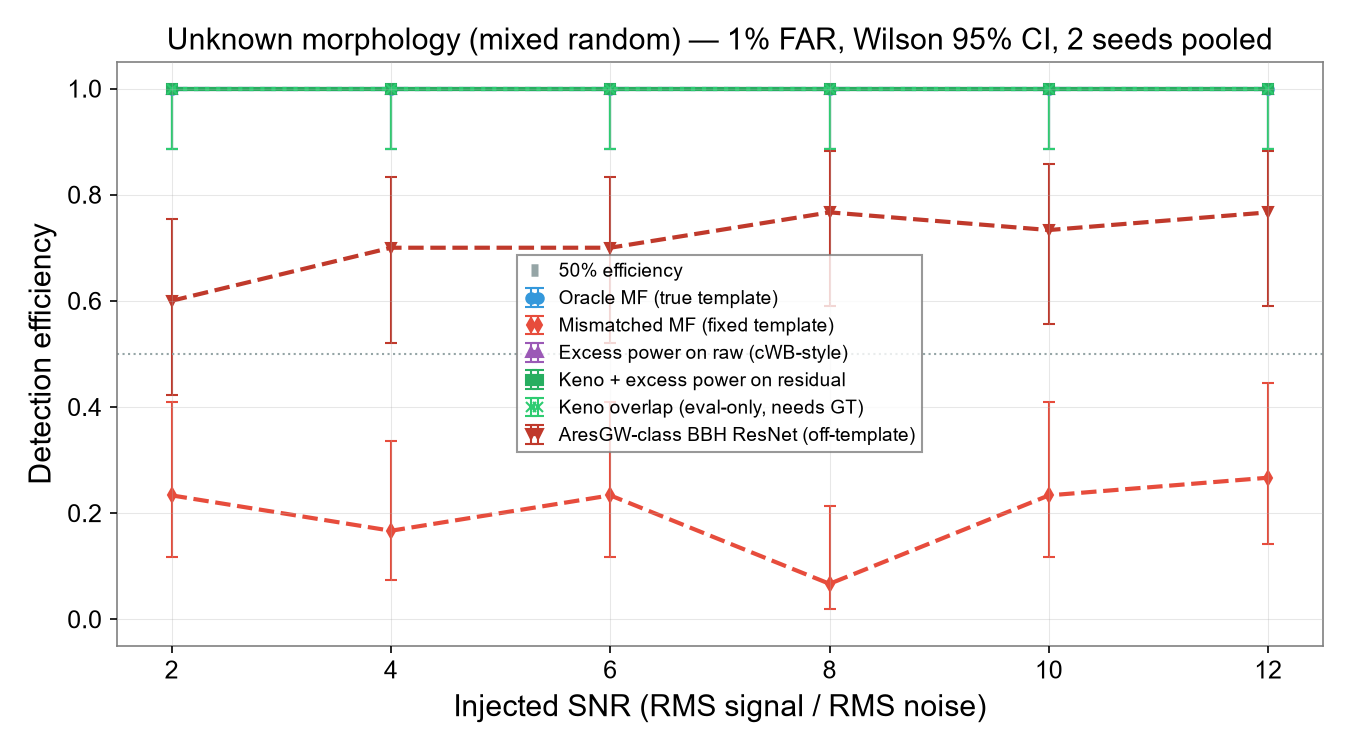
\includegraphics[width=0.95\linewidth]{figures/fig2_efficiency.png}
  \caption{Detection efficiency vs injected SNR at 1\% FAR on unknown morphology.
  AresGW-class is evaluated off-template.}
  \label{fig:eff}
\end{figure}

\begin{figure}[t]
  \centering
  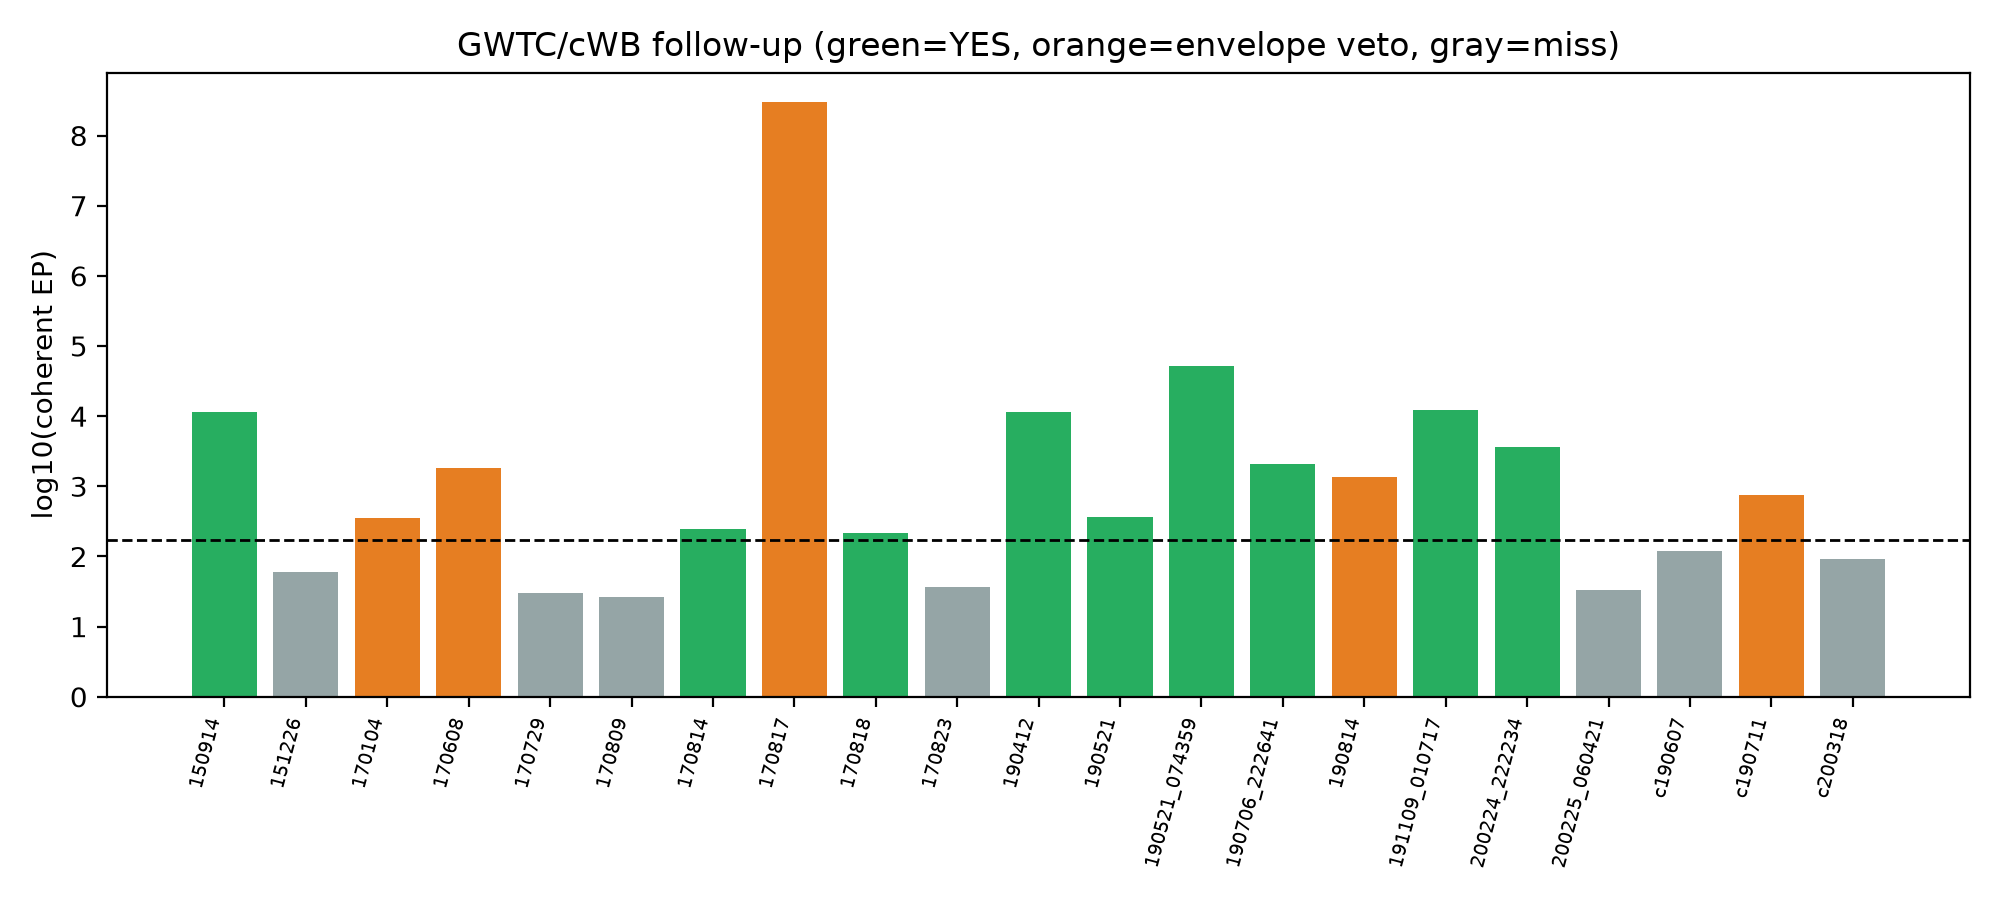
\includegraphics[width=0.95\linewidth]{figures/fig5_followup.png}
  \caption{Follow-up coherent EP by event. Green: production YES; orange: envelope veto; gray: miss.}
  \label{fig:followup}
\end{figure}

\section{Discussion}

Keno and AresGW answer different questions. Use AresGW (or matched filtering)
for BBH CBC in-band; use Keno when the waveform family is unknown.
Limitations include near-zero single-IFO glitch kill rate (coincidence and
envelope veto are the defense), residual over-subtraction risk (mitigated by
fine-tuning and validation), and incomplete recovery of cWB-only candidates.

\section{Reproducibility}

Frozen artifacts live under \texttt{docs/freeze/current/} with checkpoint SHA256
\texttt{55ce7637\ldots} (label \texttt{2026-07-paper-v1}).
Reproduce with:
\begin{verbatim}
cd ml-engine
python -m app.evaluation.aresgw_class --train
python -m app.prove --freeze --freeze-label 2026-07-paper-v1
\end{verbatim}

\section{Conclusion}

Generative noise subtraction with template-free coherent residual search
recovers unknown-morphology bursts where BBH-trained classifiers fail, at
controlled false-alarm rate, without claiming BBH superiority over AresGW.

\section*{Data availability}
Code and freeze bundle accompany this manuscript. Large evaluation CSVs are
hashed in the freeze manifest.

\bibliographystyle{plainnat}
\begin{thebibliography}{99}

\bibitem[Nousi et~al.(2023)]{nousi2023}
P.~Nousi et~al.,
\newblock Deep residual networks for gravitational wave detection,
\newblock Phys.\ Rev.\ D \textbf{108}, 024022 (2023).

\bibitem[Koloniari et~al.(2025)]{koloniari2025}
A.~E.~Koloniari et~al.,
\newblock New gravitational wave discoveries enabled by machine learning,
\newblock Mach.\ Learn.: Sci.\ Technol.\ (2025).

\bibitem[Ronneberger et~al.(2015)]{ronneberger2015}
O.~Ronneberger, P.~Fischer, and T.~Brox,
\newblock U-Net: Convolutional networks for biomedical image segmentation,
\newblock in Medical Image Computing and Computer-Assisted Intervention
(MICCAI), pp.~234--241, Springer (2015).

\end{thebibliography}
\end{document}
